%\documentclass[first=dgreen,second=purple,logo=yellowexc]{aaltoslides}
\documentclass{beamer}
%\documentclass{aaltoslides} % DEFAULT
%\documentclass[first=purple,second=lgreen,logo=redque,normaltitle,nofoot]{aaltoslides} % SOME OPTION EXAMPLES

\usepackage[latin9]{inputenc}
\usepackage[T1]{fontenc}
\usepackage{graphicx}
\usepackage{amssymb,amsmath}
\usepackage{url}
\usepackage{lastpage}
\setbeamercovered{transparent}

\usepackage[SCI]{aaltologo}


\usepackage{scrextend}
\changefontsizes{10pt}


\newcommand{\bmx}[0]{\begin{bmatrix}}
\newcommand{\emx}[0]{\end{bmatrix}}
\newcommand{\qt}[1]{\left<#1\right>}
\newcommand{\qexp}[1]{\left<#1\right>}
\newcommand{\qlay}[1]{\left[#1\right]}
\newcommand{\vect}[1]{\mathbf{#1}}
\newcommand{\vects}[1]{\boldsymbol{#1}}
\newcommand{\matr}[1]{\mathbf{#1}}
\newcommand{\var}[0]{\operatorname{Var}}
\newcommand{\cov}[0]{\operatorname{Cov}}
\newcommand{\diag}[0]{\operatorname{diag}}
\newcommand{\matrs}[1]{\boldsymbol{#1}}
\newcommand{\va}[0]{\vect{a}}
\newcommand{\vb}[0]{\vect{b}}
\newcommand{\vc}[0]{\vect{c}}
\newcommand{\vh}[0]{\vect{h}}
\newcommand{\vv}[0]{\vect{v}}
\newcommand{\vf}[0]{\vect{f}}
\newcommand{\vx}[0]{\vect{x}}
\newcommand{\vy}[0]{\vect{y}}
\newcommand{\vg}[0]{\vect{g}}
\newcommand{\vr}[0]{\vect{r}}
\newcommand{\vq}[0]{\vect{q}}
\newcommand{\vm}[0]{\vect{m}}
\newcommand{\vs}[0]{\vect{s}}
\newcommand{\vw}[0]{\vect{w}}
\newcommand{\vL}[0]{\vect{L}}
\newcommand{\vp}[0]{\vect{p}}
\newcommand{\mW}[0]{\matr{W}}
\newcommand{\mG}[0]{\matr{G}}
\newcommand{\mX}[0]{\matr{X}}
\newcommand{\mY}[0]{\matr{Y}}
\newcommand{\mK}[0]{\matr{K}}
\newcommand{\mH}[0]{\matr{H}}
\newcommand{\mQ}[0]{\matr{Q}}
\newcommand{\mU}[0]{\matr{U}}
\newcommand{\mR}[0]{\matr{R}}
\newcommand{\mV}[0]{\matr{V}}
\newcommand{\mA}{\matr{A}}
\newcommand{\mD}{\matr{D}}
\newcommand{\mC}{\matr{C}}
\newcommand{\mS}{\matr{S}}
\newcommand{\mI}{\matr{I}}
\newcommand{\mL}{\matr{L}}
\newcommand{\mzero}[0]{\matr{0}}
\newcommand{\td}[0]{\text{d}}
\newcommand{\valpha}[0]{\vects{\alpha}}
\newcommand{\vbeta}[0]{\vects{\beta}}
\newcommand{\vsig}[0]{\vects{\sigma}}
\newcommand{\vmu}[0]{\vects{\mu}}
\newcommand{\vone}[0]{\vects{1}}
\newcommand{\vzero}[0]{\vects{0}}
%\newcommand{\tf}[0]{\text{f}}
\newcommand{\tf}[0]{\text{m}}
\newcommand{\tdf}[0]{\text{dm}}
\newcommand{\TT}[0]{{\vects{\theta}}}
\newcommand{\grad}[0]{\nabla}
\newcommand{\N}[0]{\mathcal{N}}
\newcommand{\CC}[0]{\mathcal{C}}
\newcommand{\QQ}[0]{\mathbb{Q}}
\newcommand{\PP}[0]{\mathbb{P}}
\newcommand{\RR}[0]{\mathbb{R}}
\newcommand{\NN}[0]{\mathcal{N}}
\newcommand{\MM}[0]{\mathcal{M}}
\newcommand{\LL}[0]{\mathcal{L}}
\newcommand{\HH}[0]{\mathcal{H}}
\newcommand{\T}[0]{\mathcal{T}}
\newcommand{\BB}[0]{\mathcal{B}}
\newcommand{\KL}[0]{\text{KL}}
\newcommand{\CD}[0]{\text{CD}}
\newcommand{\sigmoid}{\sigma}
\newcommand{\E}[0]{\mathbb{E}}
\newcommand{\enabla}[0]{\ensuremath{%
    \overset{\raisebox{-0.3ex}[0.5ex][0ex]{%
    \ensuremath{\scriptscriptstyle e}}}{\nabla}}}
\newcommand{\enhnabla}[0]{\nabla_{\hspace{-0.5mm}e}\,}
\newcommand{\tred}[1]{\textcolor{red}{#1}}
\newcommand{\tblue}[1]{\textcolor{blue}{#1}}
\newcommand{\dd}[1]{\text{d}{#1}}

\DeclareMathOperator*{\argmin}{arg\,min}
\DeclareMathOperator*{\argmax}{arg\,max}

\newcommand{\dbm}{DBM}
\newcommand{\dbmptrbm}{DBM$^\text{DBN}_\text{RBM}$}
\newcommand{\dbmptdae}{DBM$^\text{sDAE}_\text{RBM}$}
\newcommand{\dbmptruslan}{DBM$^\text{S\&H}$}
\newcommand{\dbmptruslanrbm}{DBM$^\text{S\&H}_\text{RBM}$}
\newcommand{\dbmptruslanfvbm}{DBM$^\text{S\&H}_\text{FVBM}$}

\title{Learning and Inference in \\ Deep, Unsupervised Neural Networks}

\author[K. Cho]{Kyunghyun Cho}
\institute[ICS]{Department of Information and Computer Science\\
Aalto University, School of Science\\kyunghyun.cho@aalto.fi}

%\aaltofootertext{Foundations and Advances in Deep Learning}{\today}{\arabic{page}/\pageref{LastPage}\ }

\date{21 March 2014}

\begin{document}

%%%%%%%%%%%%%%%%%%%%%%%%%%%%%%%%%%%%%%%%%%%%%%%%%%%%%%%%%%%%%%%%%%%%%%%%%%%%%%%%%%%%%%%%%%%%%

\frame{\titlepage}
%\aaltotitleframe

%%%%%%%%%%%%%%%%%%%%%%%%%%%%%%%%%%%%%%%%%%%%%%%%%%%%%%%%%%%%%%%%%%%%%%%%%%%%%%%%%%%%%%%%%%%%%

\begin{frame}
    \raggedright
    This work was done under the supervision of Prof. Juha
    Karhunen, Prof. Tapani Raiko and Dr. Alexander Ilin at
    the Deep Learning and Bayesian Modeling Group,
    Department of Information and Computer Science, Aalto
    University School of Science between mid 2009 and early 2014.

    \vspace{10mm}
    \raggedleft
    \AaltoLogoSmall{0.5}{!}{aaltoRed}

\end{frame}

\begin{frame}
    \tableofcontents[ 
    currentsubsection, 
    %hideothersubsections, 
    sectionstyle=show, 
    subsectionstyle=show,
    ] 
\end{frame}

\section{Introduction}

\subsection{Machine Learning}

\begin{frame}{Machine Learning in a Single Slide}
    \centering
    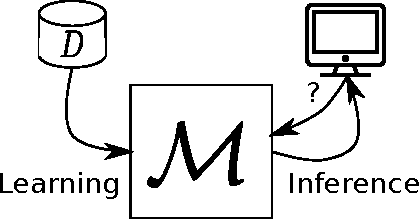
\includegraphics[width=0.55\textwidth]{machinelearning.pdf}

    \vspace{4mm}
    \raggedright
    \begin{enumerate}
        \item Let the model $\MM$ \tred{\textit{learn}} the data $D$
        \item Let the model $\MM$ \tblue{\textit{infer}} unknown
            quantities
    \end{enumerate}
\end{frame}

\begin{frame}{Examples}
    \centering
    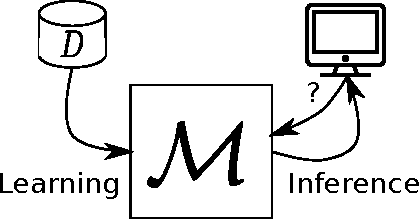
\includegraphics[width=0.55\textwidth]{machinelearning.pdf}

    \vspace{3mm}
    \begin{center}
    { \small
    \begin{tabular}{l | l}
        Data & Query \\
        \hline
        \hline
        Movie Ratings & 
        Will a user $X$ like a movie $Y$? \\
        Tagged Images &
        Is a cat in this image?  \\
        Transcribed Speech &
        What is this person saying?  \\
        Parallel Corpora &
        What is ``moi'' in English?  
    \end{tabular}
    }
\end{center}
\end{frame}

\subsection{Deep Learning}

\begin{frame}{Deep Learning in a Single Slide}

    \vfill

     \centering
     \begin{minipage}{0.32\textwidth}
         \centering
         
\includegraphics[width=0.9\columnwidth]{studying.pdf}
     \end{minipage}
     \hfill
     \begin{minipage}{0.32\textwidth}
         \centering
         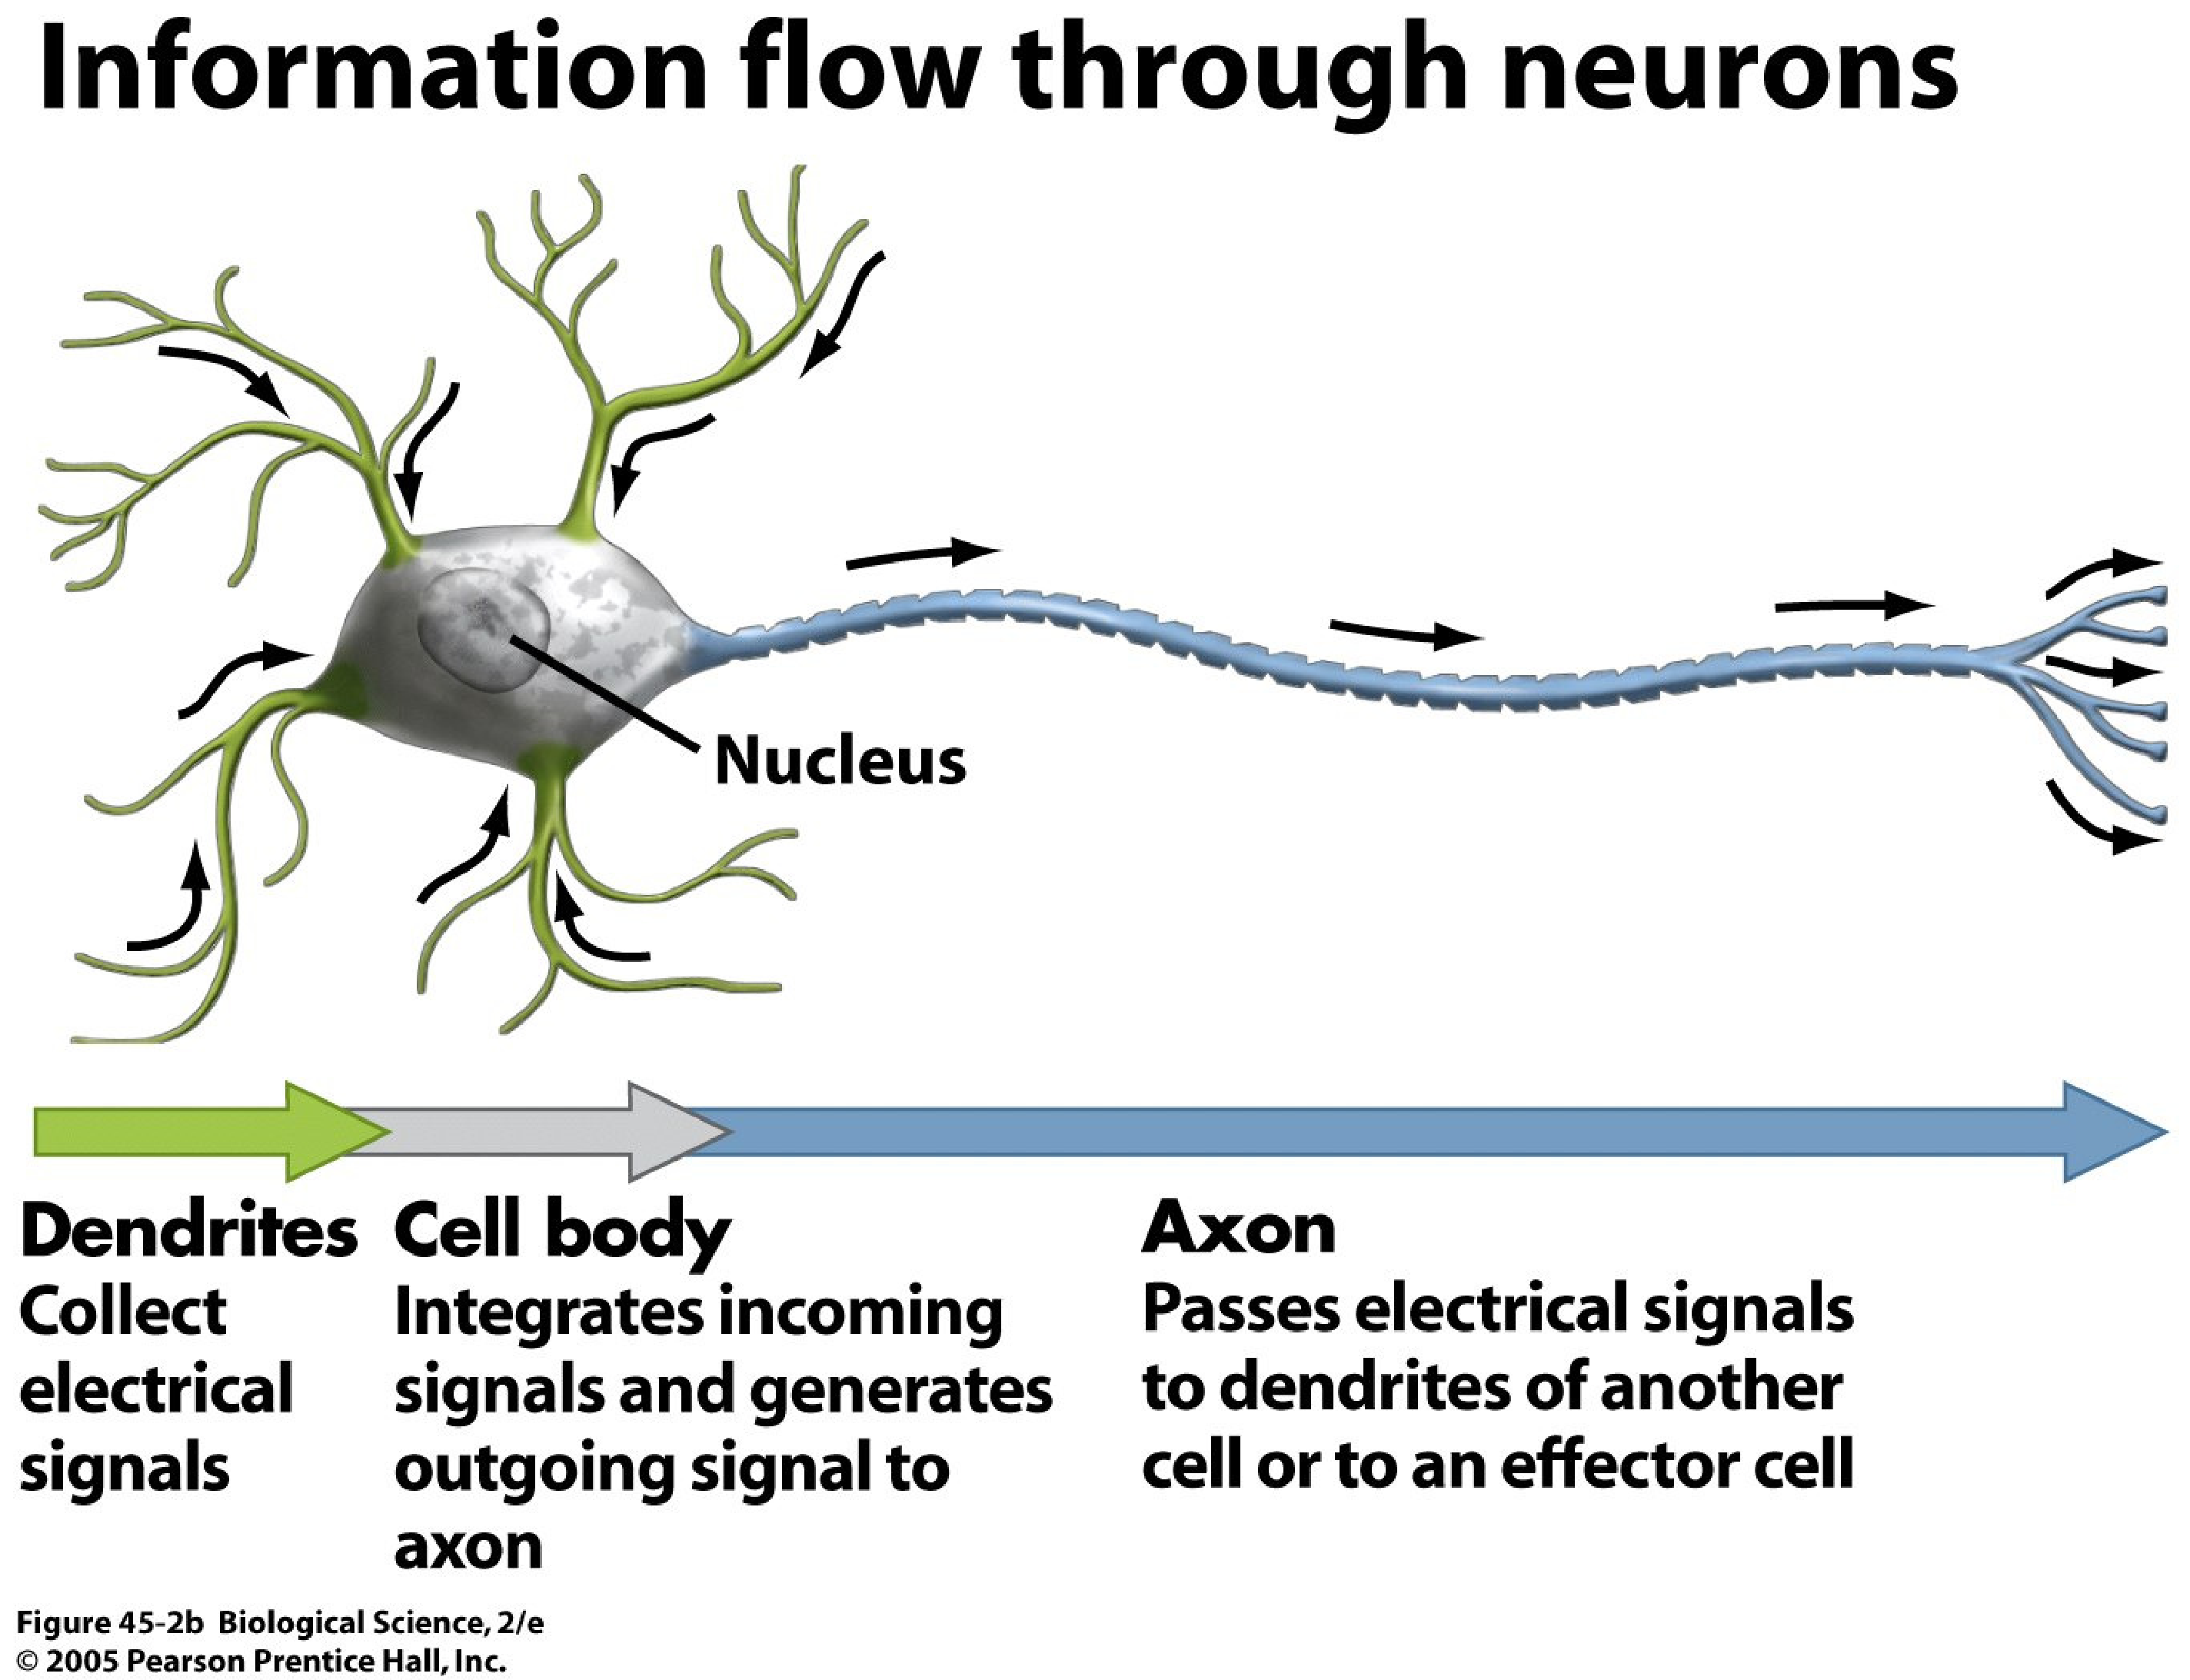
\includegraphics[width=0.9\columnwidth]{neuron.pdf}
     \end{minipage}
     \hfill
     \begin{minipage}{0.32\textwidth}
         \centering
         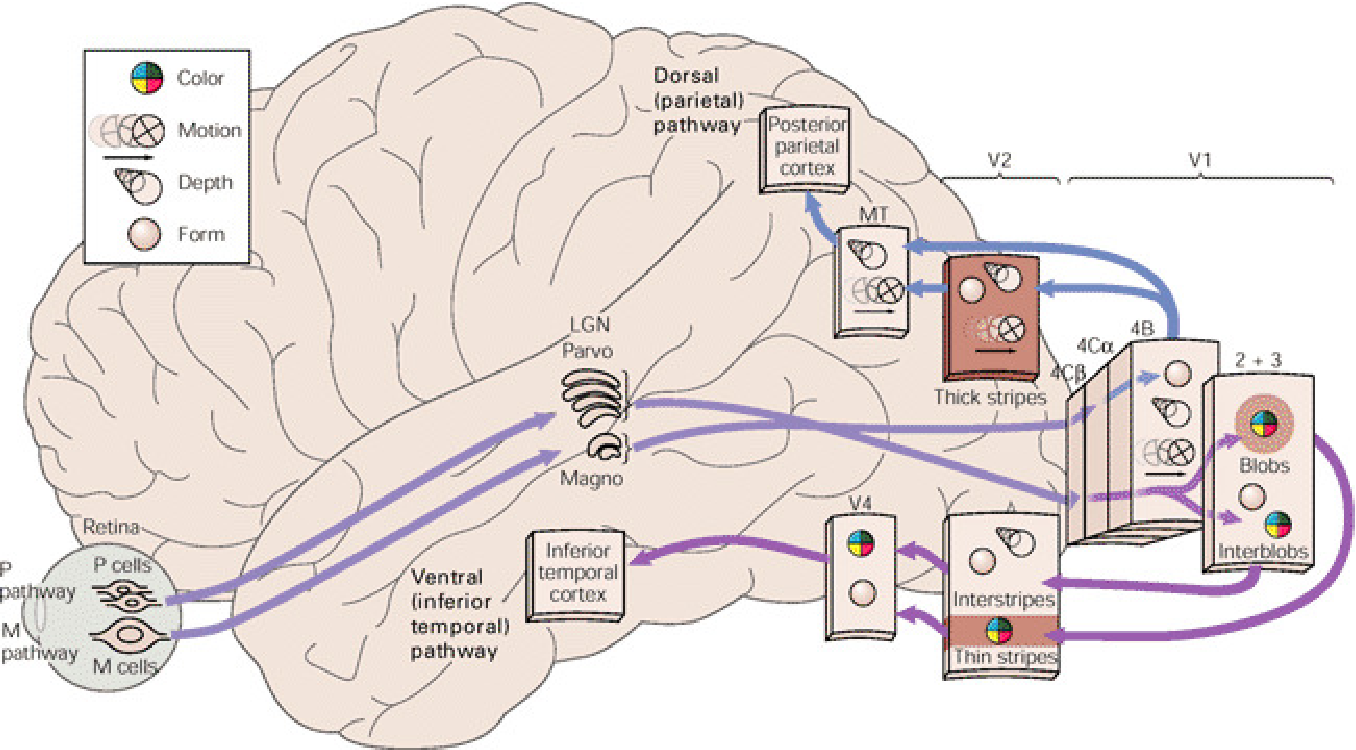
\includegraphics[width=0.9\columnwidth]{visual_pathway.pdf}
         \\
         \raggedleft {\tiny (Van Essen\&Gallant, 1994)}
     \end{minipage}

     \begin{minipage}{0.32\textwidth}
         \centering
         \small
         \textit{Learn} massive data
     \end{minipage}
     \hfill
     \begin{minipage}{0.32\textwidth}
         \centering
         \small
         \textit{simple functions}
     \end{minipage}
     \hfill
     \begin{minipage}{0.32\textwidth}
         \centering
         \small
         \textit{Multi-layered} 
     \end{minipage}

     \vspace{3mm}
    \centering
    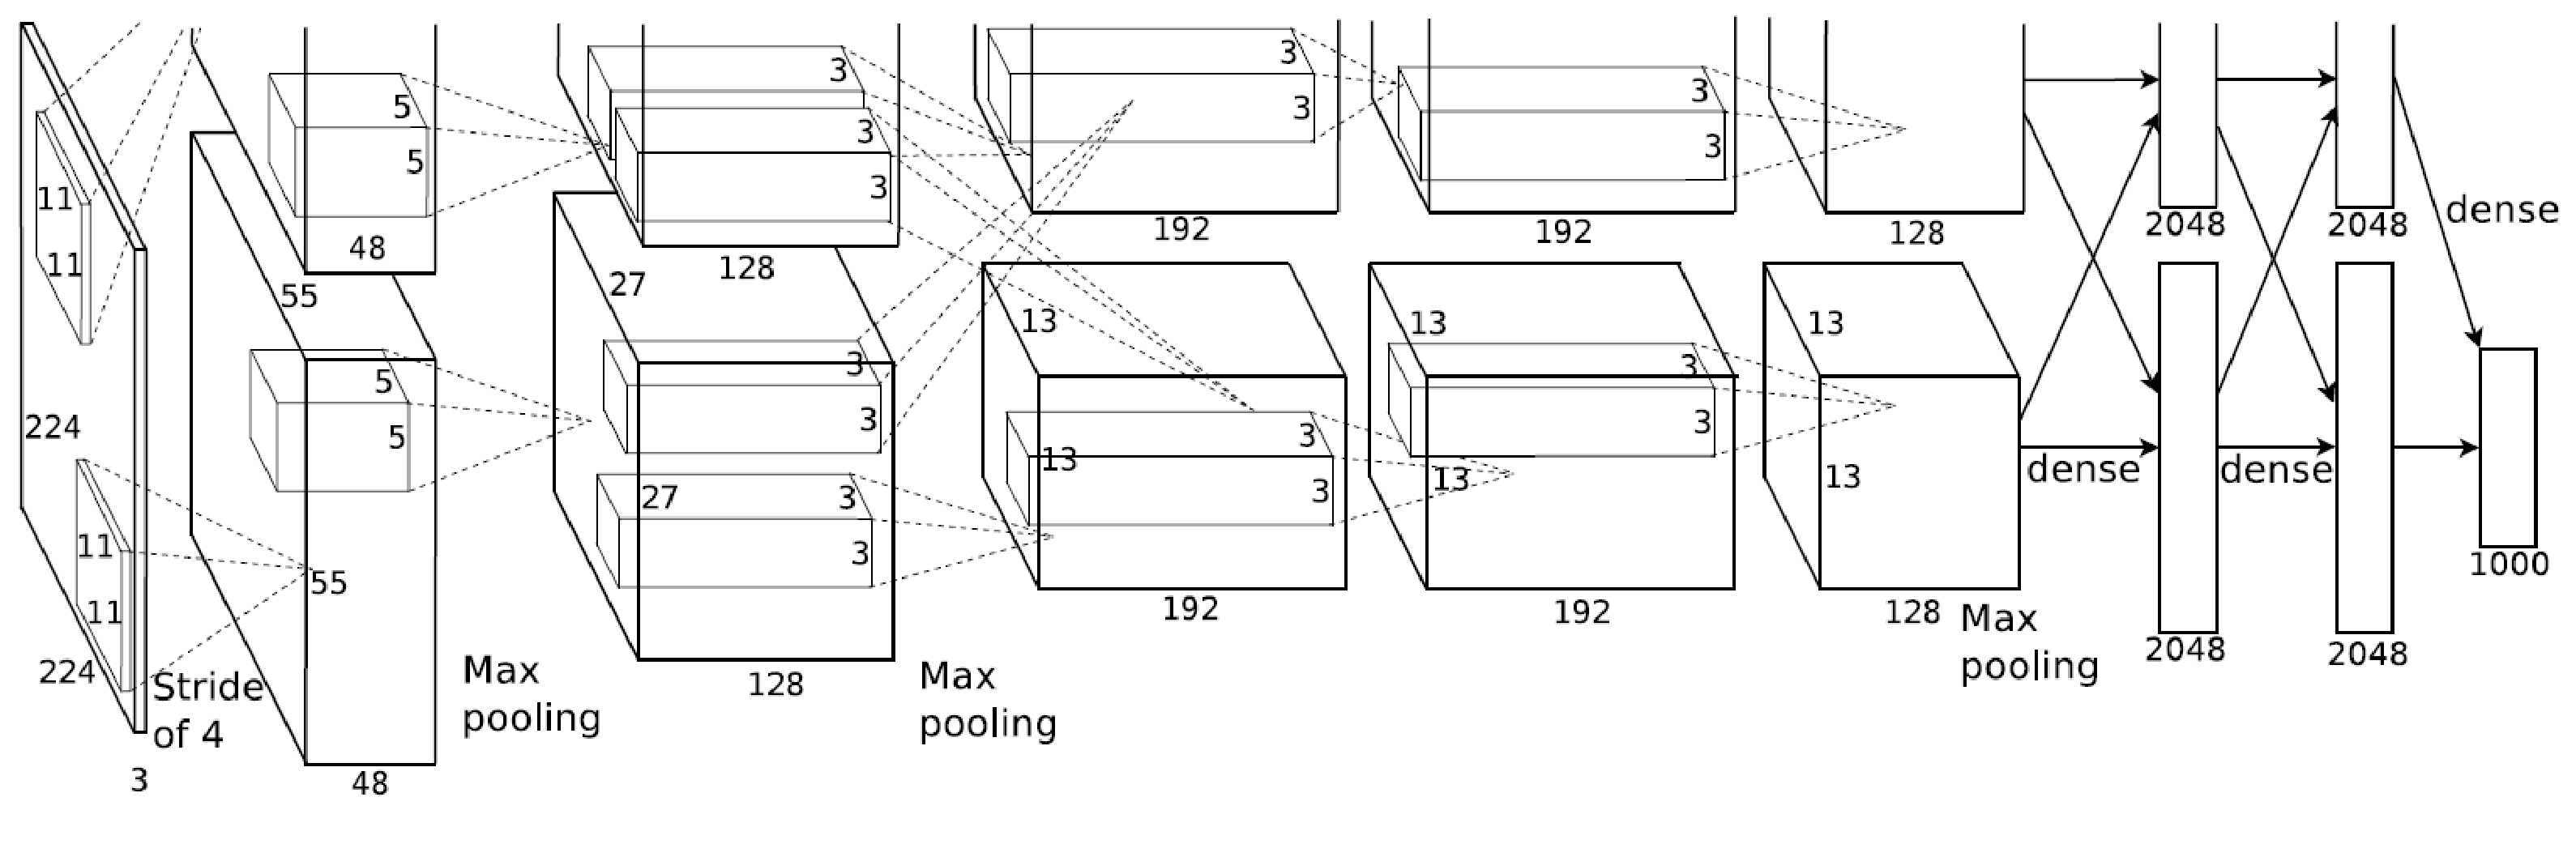
\includegraphics[width=0.8\textwidth]{alex_imagenet}
    \\
    \raggedleft {\tiny (Krizhevsky et al., 2012)}

    \vfill


\end{frame}

\subsection{Challenges}

\begin{frame}{Challenges in Machine Learning}
    \centering
    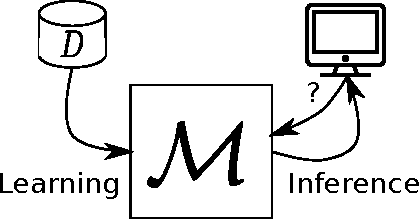
\includegraphics[width=0.55\textwidth]{machinelearning.pdf}

    \vspace{4mm}
    \raggedright
    \begin{enumerate}
        \item \tred{Learning} is \emph{not} trivial 
        \item \tred{Learning} and \tblue{inference} are \emph{not} separate
    \end{enumerate}
\end{frame}

\begin{frame}{Is Learning Optimization?}

    \centering
    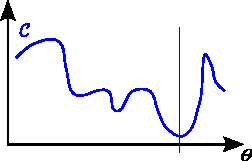
\includegraphics[width=0.5\textwidth]{cost_true.pdf}

    \begin{minipage}{0.48\textwidth}
        \textbf{\emph{Yes}}
    \end{minipage}
    \hfill
    \begin{minipage}{0.48\textwidth}
    %\emph{No}
    \end{minipage}

    %\vspace{1mm}

    \begin{minipage}[t]{0.48\textwidth}
        \vspace{0pt}
    Learning minimizes a cost function $\color{blue}{\CC}$ with respect to
    $\MM$ given a data distribution $p_D$

    \end{minipage}
    \hfill
    \begin{minipage}[t]{0.48\textwidth}
    %    \vspace{0pt}
    %$\color{blue}{\CC}$ is \emph{not} available, but $\color{red}{\tilde{\CC}}$ based
    %on the samples from $p_D$.

    \end{minipage}

\end{frame}

\begin{frame}{Is Learning Optimization?}

    \centering
    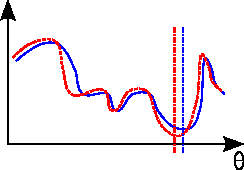
\includegraphics[width=0.5\textwidth]{cost_both.pdf}

    \begin{minipage}{0.48\textwidth}
        \textbf{\emph{Yes}}
    \end{minipage}
    \hfill
    \begin{minipage}{0.48\textwidth}
        \textbf{\emph{No}}
    \end{minipage}

    %\vspace{1mm}

    \begin{minipage}[t]{0.48\textwidth}
        \vspace{0pt}
    Learning minimizes a cost function $\color{blue}{\CC}$ with respect to
    $\MM$ given a data distribution $p_D$

    \end{minipage}
    \hfill
    \begin{minipage}[t]{0.48\textwidth}
        \vspace{0pt}
    $\color{blue}{\CC}$ is \emph{not} available, but $\color{red}{\tilde{\CC}}$ based
    on the samples from $p_D$.

    \end{minipage}

\end{frame}

\begin{frame}{Vicious Cycle or Virtuous Cycle?}

    %\begin{minipage}{0.48\textwidth}
        \centering
        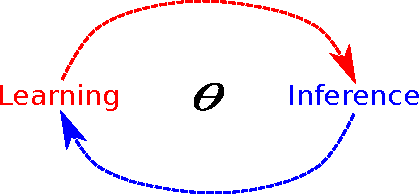
\includegraphics[width=0.5\textwidth]{vicious_cycle.pdf}
    %\end{minipage}
    %\hfill
    %\begin{minipage}{0.48\textwidth}
    %    \tred{\emph{Learning}} which changes $\TT$ requires
    %    \tblue{\emph{inferences}} based on $\TT$. 
    %\end{minipage}

    \vfill
    \raggedright
    Example: MLE for feedforward neural networks
    \begin{align*}
        {\color{red} \min_{\TT} \CC(\TT)} \approx 
        {\color{red} \min_{\TT} \tilde{\CC}(\TT)} =
        {\color{red} \min_{\TT} -\frac{1}{N}\sum_{\left(\vx,t\right) \in D}
        \log {\color{blue}p(y=t \mid \vx, \TT)}}
    \end{align*}

\end{frame}

\begin{frame}{What gets worse with \emph{deep} learning?}
    \begin{itemize}
        \item Learning/Optimization 
            \begin{itemize}
                \item No access to $\CC$, but only to $\tilde{\CC}$
                \item Highly entangled inference and learning
                \item \textbf{High-dimensional}
                \item \textbf{Non-convex with a lot of local (apparent) minima}
                \item \textbf{Often, intractable to compute
                    even $\tilde{\CC}$}
            \end{itemize}
    \end{itemize}

    \begin{itemize}
        \item Inference
            \begin{itemize}
                \item \textbf{No analytical expression}, often
                \item \textbf{Intractable to compute}, often
            \end{itemize}
    \end{itemize}
\end{frame}

\section{Deep, Unsupervised Neural Networks}

\begin{frame}{}
    \begin{center}
    Deep, Unsupervised Neural Networks \\
    Boltzmann Machines and Autoencoders
\end{center}

{\scriptsize
\begin{enumerate}
    \item[\textbf{I}] Enhanced
Gradient for Training Restricted Boltzmann Machines

    \item[\textbf{II}] Enhanced Gradient and Adaptive
        Learning Rate for Training Restricted Boltzmann
        Machines

\item[\textbf{III}] 
Parallel Tempering is Efficient for Learning Restricted Boltzmann Machines

\item[\textbf{VII}] A Two-Stage Pretraining Algorithm for
Deep Boltzmann Machines

\item[\textbf{VIII}] Simple Sparsification Improves Sparse Denoising Autoencoders
in Denoising Highly Corrupted Images
\end{enumerate}
}

\end{frame}

\subsection{Restricted Boltzmann Machines}

\begin{frame}{Boltzmann Machines}

    \begin{minipage}{0.33\textwidth}
        \begin{minipage}{\columnwidth}
            \centering
            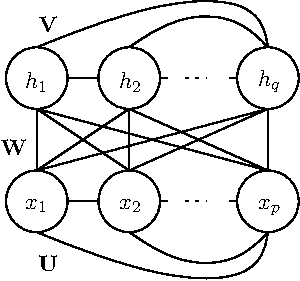
\includegraphics[width=0.99\columnwidth]{boltzmann.pdf}
        \end{minipage}
        
        \vspace{3mm}

        \begin{minipage}{\columnwidth}
            \small 
            \begin{itemize}
                \item If $\mV=\mzero$ and $\mU=\mzero$, restricted Boltzmann
                    machine (RBM)
                \item If $\mU=\mzero$ and layered $\vh$, deep Boltzmann
                    machine (DBM)
            \end{itemize} 
        \end{minipage}
    \end{minipage}
    \hfill
    \begin{minipage}{0.65\textwidth}
        \small
        \begin{enumerate}
            \item Negative energy over $\vx$ and $\vh$:
                \begin{align*}
                -E(\vx, \vh &\mid \TT) = \vb^\top \vx +
                \vc^\top \vh + \\
                &
                \vx^\top \mW \vh + \frac{1}{2} \vx^\top \mU \vx +
                \frac{1}{2} \vh^\top \mV \vh
            \end{align*}
            \item Probability over $\vx$ and
                $\vh$:
                \begin{align*}
                p(\vx, \vh \mid \TT) = \frac{1}{Z(\TT)} \exp \left\{
                -E\left(\vx , \vh \mid \TT\right)
                \right\}
            \end{align*}
            \item Learn $p(\vx)$ by minimizing
                \begin{align*}
                    -\LL(\TT) =& -\E_{\vx \in D} \left[ \log
                    \frac{1}{Z(\TT)} \sum_{\vh}
                    e^{-E\left( \vx, \vh \mid \TT\right)}
    \right]
            \end{align*}
            with stochastic gradient descent
        \end{enumerate}
    \end{minipage}
\end{frame}

\begin{frame}{Learning: Observations}
    \begin{minipage}{0.59\textwidth}
        \begin{center}
            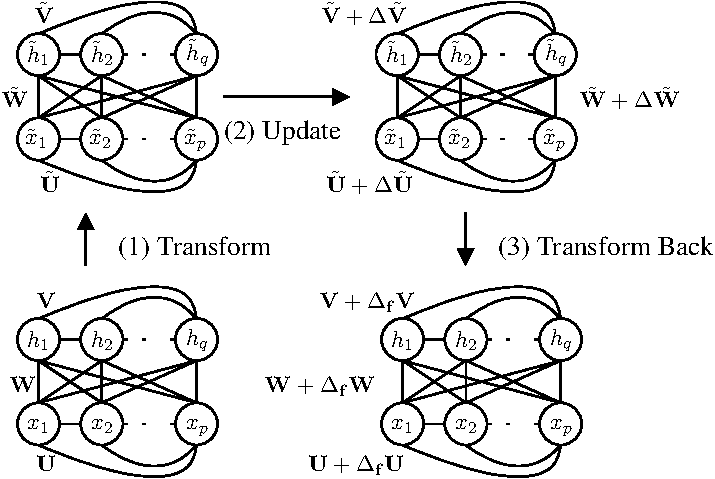
\includegraphics[width=\textwidth]{transf.pdf}
        \end{center}
    \end{minipage}
    \hfill
    \begin{minipage}{0.4\textwidth}
        \small 
        \begin{itemize}
            \item Invariant to bit-flipping transformation
            \item $2^{p+q}$ descent directions 
            \item leading to (potentially all) different solutions
            \item Which direction?
            \item How to tractably decide?
        \end{itemize}
    \end{minipage}
\end{frame}

\begin{frame}{Learning: Enhanced Gradient}
    \begin{minipage}{0.35\textwidth}
        \begin{minipage}{\columnwidth}
            \begin{center}
                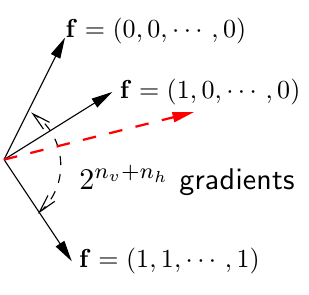
\includegraphics[width=0.6\textwidth]{enhgrad.png}
            \end{center}
        \end{minipage}

        \vspace{2mm}

        \begin{minipage}{\columnwidth}
            \scriptsize
            \begin{center}
                Covariance of Weight Updates
            \end{center}
        \end{minipage}
        \\
        \begin{minipage}{0.49\columnwidth}
            \begin{minipage}{\columnwidth}
                \begin{center}
                    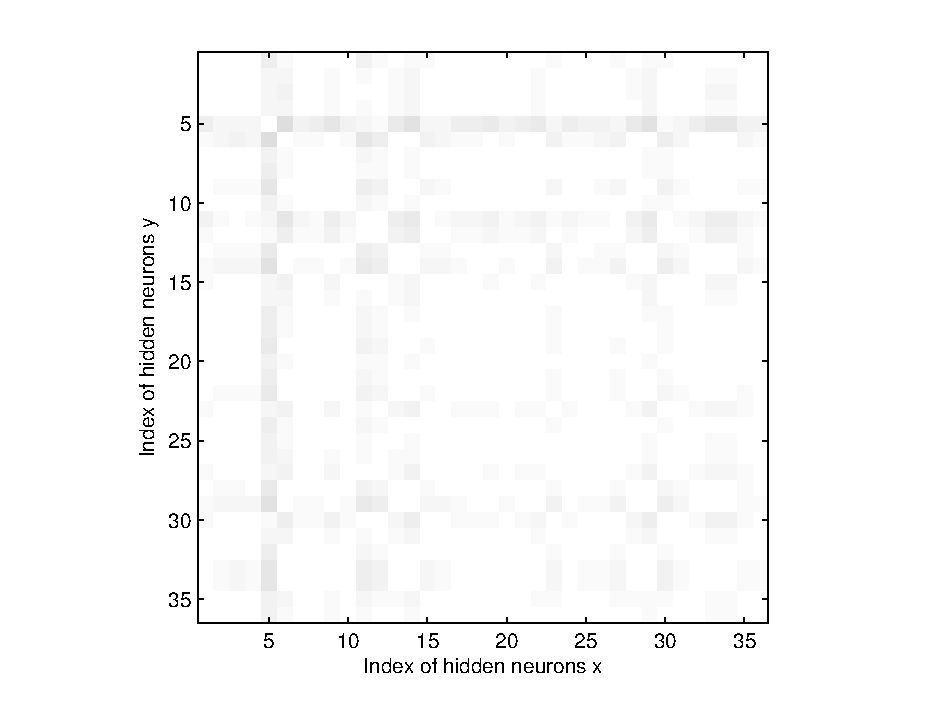
\includegraphics[width=\columnwidth,trim=93 35 75 20,clip=true]{norm_grad_cov.pdf}
                \end{center}
            \end{minipage}
            \begin{minipage}{\columnwidth}
                \begin{center}
                    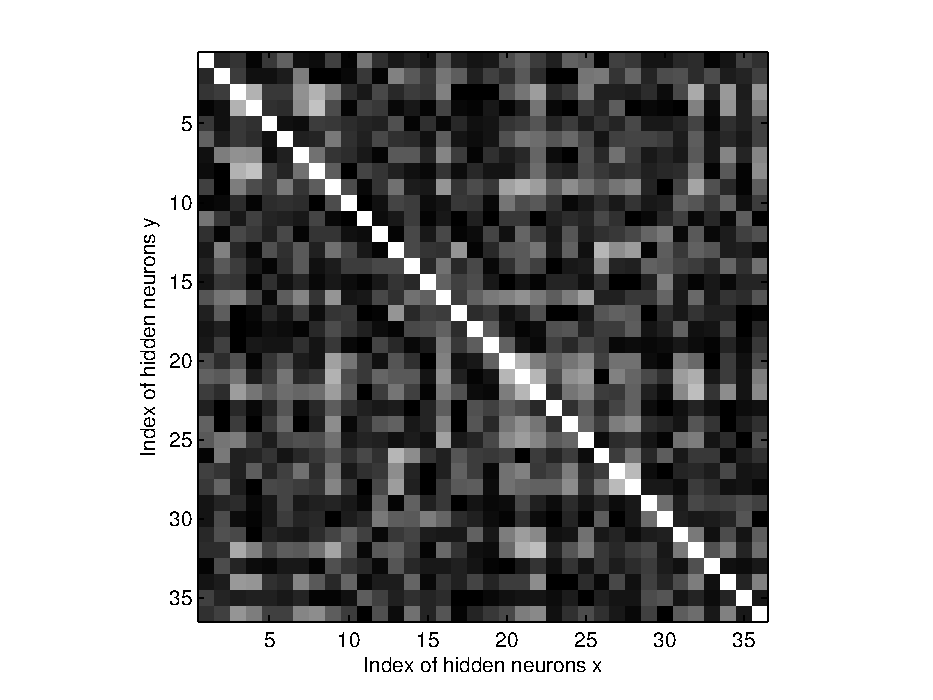
\includegraphics[width=\columnwidth,trim=93 35 75 20,clip=true]{enh_grad_cov.pdf}
                \end{center}
            \end{minipage}
        \end{minipage}
        \hfill
        \begin{minipage}{0.49\columnwidth}
            \begin{minipage}{\columnwidth}
                \begin{center}
                    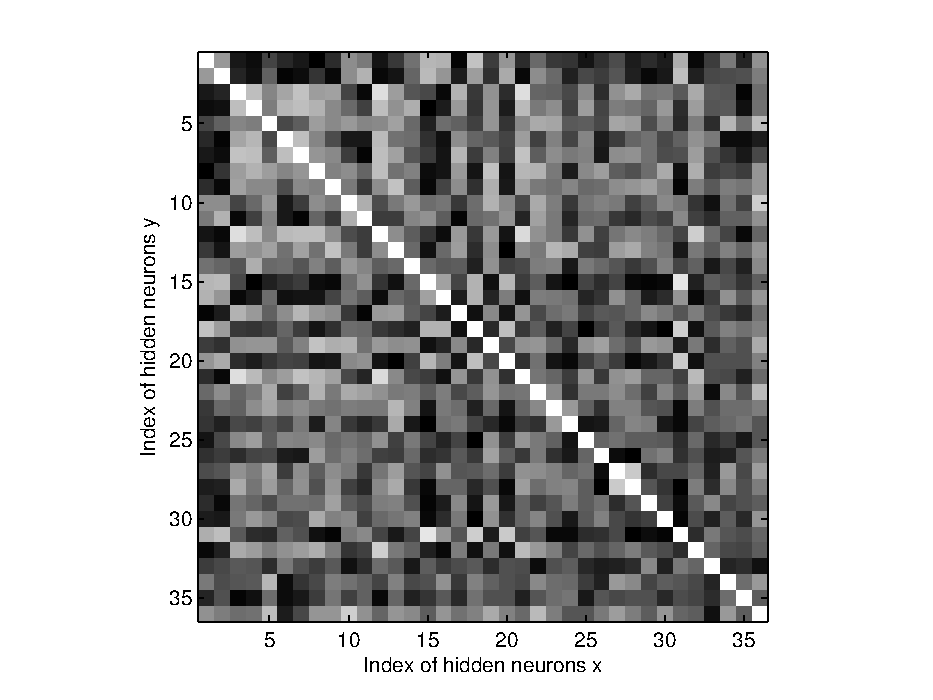
\includegraphics[width=\columnwidth,trim=93 35 75 20,clip=true]{norm_grad_cov_later.pdf}
                \end{center}
            \end{minipage}
            \begin{minipage}{\columnwidth}
                \begin{center}
                    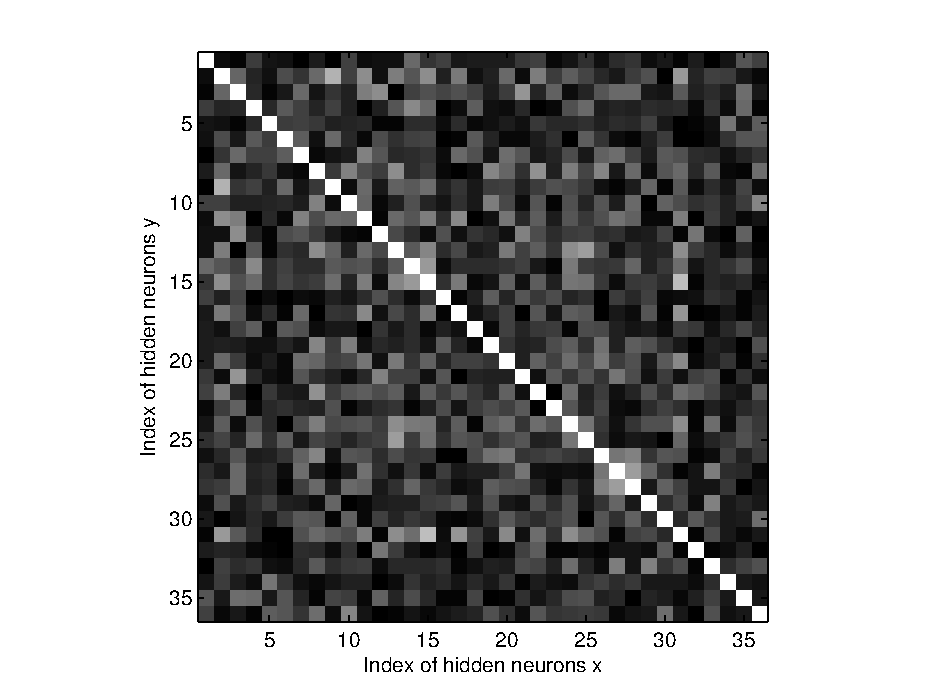
\includegraphics[width=\columnwidth,trim=93 35 75 20,clip=true]{enh_grad_cov_later.pdf}
                \end{center}
            \end{minipage}
        \end{minipage}
        \\
        \begin{minipage}{0.49\columnwidth}
            \scriptsize
            \begin{center}
                Conventional
            \end{center}
        \end{minipage}
        \hfill
        \begin{minipage}{0.49\columnwidth}
            \scriptsize
            \begin{center}
                Enhanced
            \end{center}
        \end{minipage}
    \end{minipage}
    \hfill
    \begin{minipage}{0.64\textwidth}
        \small 
        \begin{itemize}
            \item Importance weight of each direction $\nabla_{\vf} \LL$
                \begin{align*}
                    \prod_{k=1}^{n_v+n_h} \qexp{x_k}_\tdf^{f_k}
                    \left( 1 - \qexp{x_k}_\tdf
                    \right)^{1-f_k} 
                \end{align*}

            \item Weighted sum of all possible updates 
            \begin{align*}
                \enhnabla w_{ij} &= \cov_\td\left(x_i, h_j\right)
                - \cov_\tf\left(x_i, h_j\right)
                \\
                \enhnabla b_i &= \left<x_i\right>_\td - \left<x_i\right>_\tf
                - \sum_j \qexp{ h_j }_\tdf
                \enhnabla w_{ij}
                \\
                \enhnabla c_j &= \left<h_j\right>_\td - \left<h_j\right>_\tf
                - \sum_i \qexp{ x_i }_\tdf
                \enhnabla w_{ij}
            \end{align*}
        \end{itemize}
    \end{minipage}
\end{frame}

\begin{frame}{Learning vs. Inference}
    Boltzmann machine \tred{learning} requires
    \tblue{inference}.
    \begin{align*}
        {\color{red} \enhnabla w_{ij}} &= {\color{black}\cov_\td\left(x_i,
        h_j\right)}
        - {\color{blue}\cov_\tf\left(x_i, h_j\right)}
    \end{align*}

    \begin{itemize}
        \item \emph{What is the covariance between $x_i$ and $h_j$ with the
    current $\TT$?} 
    \begin{itemize}
        \item NP-Hard problem even in the case of RBMs {\small (Long\&Servedio, 2010)}
        \item Monte Carlo approximation with persistent MCMC
            \[
            {\color{blue}\cov_\tf\left(x_i, h_j\right)}
            \approx
            \left(\frac{1}{N} \sum_{n=1}^N x_i^{(n)}
            h_j^{(n)}\right) - 
            \left( 
            \frac{1}{N} \sum_{n=1}^N x_i^{(n)} 
            \right)
            \left(\frac{1}{N}
            \sum_{n=1}^N h_j^{(n)}
            \right)
            \]
        \item Gibbs sampling
    \end{itemize}
    \end{itemize}
\end{frame}

\begin{frame}{Learning vs. Inference: Vicious Cycle}

    \begin{center}
        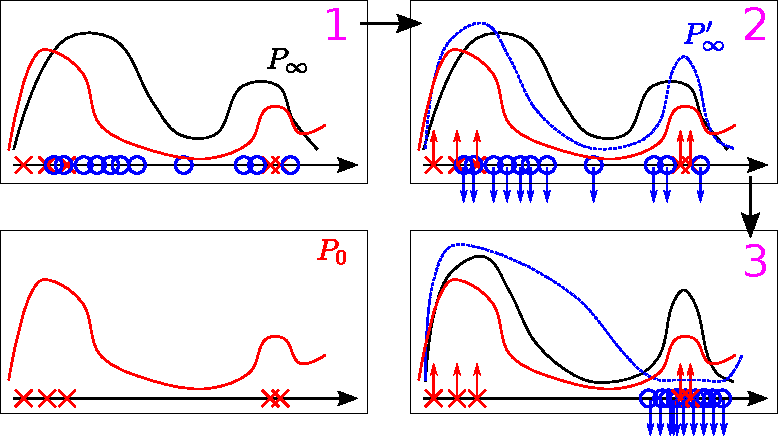
\includegraphics[width=0.9\textwidth]{vicious_cycle_bm.pdf}
    \end{center}

    \raggedright
    Failed \tblue{inference} (sampling) breaks
            \tred{learning} 

    \raggedleft
            $\to$ \emph{Good MCMC sampler is
            needed!}

\end{frame}

\begin{frame}{Inference: Parallel Tempering}
    \tred{TODO}
\end{frame}

\subsection{Deep Boltzmann Machines}

\begin{frame}{Deep Boltzmann Machines}
    \alert{TODO}
\end{frame}

\begin{frame}{Learning: Two-Stage Pretraining Algorithm}
    \alert{TODO}
\end{frame}

\subsection{Deep Autoencoders}

\begin{frame}{Inference: Explicit Sparsification via Shrinkage}
    \alert{TODO}
\end{frame}


\section{Discussion}

\begin{frame}{Thank you}
    \alert{TODO}
\end{frame}



%%%%%%%%%%%%%%%%%%%%%%%%%%%%%%%%%%%%%%%%%%%%%%%%%%%%%%%%%%%%%%%%%%%%%%%%%%%%%%%%%%%%%%%%%%%%%%

%\begin{frame}{Title Page}

%\begin{itemize}
%\item The largest difference to normal Beamer slides is that the title page is produced with a special command \texttt{\textbackslash aaltotitleframe}; this command should be used as it is. \alert{Don't put it in a frame environment!!!} See \texttt{example.tex}.
%\item By default, \texttt{aaltoslides} uses a title page similar to the one in the Aalto Powerpoint templates
%\item A more traditional looking title page can be selected with the option: \texttt{normaltitle}
%\end{itemize}

%\end{frame}

%%%%%%%%%%%%%%%%%%%%%%%%%%%%%%%%%%%%%%%%%%%%%%%%%%%%%%%%%%%%%%%%%%%%%%%%%%%%%%%%%%%%%%%%%%%%%%

%\begin{frame}{Aalto Colors}

%\begin{itemize}

%\item Colors are defined with options: \texttt{first=$\star$} and \texttt{second=$\star$} where $\star$ is one of the following:\\
%{\color{aaltoyellow}yellow}, 
%{\color{aaltored}red}, 
%{\color{aaltoblue}blue}, 
%{\color{aaltogray}gray}, 
%{\color{aaltolgreen}lgreen}, 
%{\color{aaltodgreen}dgreen}, 
%{\color{aaltocyan}cyan}, 
%{\color{aaltopurple}purple}, 
%{\color{aaltomagenta}magenta}, or
%{\color{aaltoorange}orange}

%\item The first color is the primary color (titles, the footer bar, \ldots) and the second color is used in alerted texts and examples

%\item Default colors are: {\color{aaltoblue}blue} and {\color{aaltored}red}

%\item Colors can be used also with the command: \texttt{\textbackslash color\{aalto}$\star$\texttt{\}}. For example, 
%\texttt{\{\textbackslash color\{aaltocyan\}some text\}} 
%gives {\color{aaltocyan}some text}

%\item The rules for choosing colors from the Aalto color circle are not checked (two adjacent colors should not be used)

%\end{itemize}

%\end{frame}

%%%%%%%%%%%%%%%%%%%%%%%%%%%%%%%%%%%%%%%%%%%%%%%%%%%%%%%%%%%%%%%%%%%%%%%%%%%%%%%%%%%%%%%%%%%%%%

%\begin{frame}{Logo}

%\begin{itemize}
%\item \texttt{aaltoslides} supports all variations of the logo:\\[0.2cm]
%
\includegraphics[width=3cm]{Aalto_EN_ScienceandTech_13_RGB_y1.pdf} \hspace{10pt}
%
\includegraphics[width=3cm]{Aalto_EN_ScienceandTech_13_RGB_y2.pdf} \hspace{10pt}
%
\includegraphics[width=3cm]{Aalto_EN_ScienceandTech_13_RGB_y3.pdf} \\[0.2cm]
%
\includegraphics[width=3cm]{Aalto_EN_ScienceandTech_13_RGB_r1.pdf} \hspace{10pt}
%
\includegraphics[width=3cm]{Aalto_EN_ScienceandTech_13_RGB_r2.pdf} \hspace{10pt}
%
\includegraphics[width=3cm]{Aalto_EN_ScienceandTech_13_RGB_r3.pdf} \\[0.2cm]
%
\includegraphics[width=3cm]{Aalto_EN_ScienceandTech_13_RGB_b1.pdf} \hspace{10pt}
%
\includegraphics[width=3cm]{Aalto_EN_ScienceandTech_13_RGB_b2.pdf} \hspace{10pt}
%
\includegraphics[width=3cm]{Aalto_EN_ScienceandTech_13_RGB_b3.pdf} \\
%\item The logo is selected with the option: \texttt{logo=$\star\circ$} where $\star$ is {\color{aaltoyellow}yellow}, {\color{aaltored}red}, or {\color{aaltoblue}blue}, and $\circ$ is either exc, quo, or que for !, ", or ?, respectively; For example, \texttt{logo=yellowquo}
%\item The title page uses a larger variation of the selected logo
%\item By default, the logo is \texttt{logo=redexc}
%\item All logos can be removed with the option: \texttt{nologo}
%\end{itemize}

%\end{frame}

%%%%%%%%%%%%%%%%%%%%%%%%%%%%%%%%%%%%%%%%%%%%%%%%%%%%%%%%%%%%%%%%%%%%%%%%%%%%%%%%%%%%%%%%%%%%%%

%\begin{frame}{Footer}

%\begin{itemize}

%\item By default, the slides have a footer with a logo on the left and an optional three row text\footnote{The first row is highlighted with black by default. To remove this, simply change the color of the first argument of  \texttt{\textbackslash aaltofootertext\{\}\{\}\{\}} with \texttt{\textbackslash color\{aaltogray\}}} on the right
%\item The footer text is set up with the command: \texttt{\textbackslash aaltofootertext\{\}\{\}\{\}}
%\item The footer can be removed with the option: \texttt{nofoot}

%\end{itemize}

%\end{frame}

%%%%%%%%%%%%%%%%%%%%%%%%%%%%%%%%%%%%%%%%%%%%%%%%%%%%%%%%%%%%%%%%%%%%%%%%%%%%%%%%%%%%%%%%%%%%%%

%\begin{frame}{Lengths}

%\begin{itemize}
%\item \texttt{aaltoslides} defines the following lengths: 
%\texttt{\textbackslash aaltofooterplace}, 
%\texttt{\textbackslash aaltofooterruleheight}, 
%\texttt{\textbackslash aaltofooterrulewidth}, 
%\texttt{\textbackslash aaltotitleboxplace},  
%\texttt{\textbackslash aaltotitleboxheight}, 
%\texttt{\textbackslash aaltotitleboxwidth}, 
%\texttt{\textbackslash aaltotitlesep}, 
%\texttt{\textbackslash aaltotitleentrysep}, 
%\texttt{\textbackslash largelogoheight}, and
%\texttt{\textbackslash smalllogoheight} 
%\item The appearance of the slides can be changed by modifying the lengths with \texttt{\textbackslash setlength} or \texttt{\textbackslash addtolength}
%\end{itemize}

%\end{frame}

%%%%%%%%%%%%%%%%%%%%%%%%%%%%%%%%%%%%%%%%%%%%%%%%%%%%%%%%%%%%%%%%%%%%%%%%%%%%%%%%%%%%%%%%%%%%%%


%\begin{frame}{Some Examples}

%\begin{itemize}
%\item Normal text
%\item \alert{Alerted text}
%\end{itemize}

%\begin{block}{Block 1}
%Text
%\end{block}

%\begin{example}
%Text
%\end{example}

%\end{frame}

%%%%%%%%%%%%%%%%%%%%%%%%%%%%%%%%%%%%%%%%%%%%%%%%%%%%%%%%%%%%%%%%%%%%%%%%%%%%%%%%%%%%%%%%%%%%%%

\end{document}
